%%%%%%%%%%%%%%%%%%%%%%%%%%%%%%%%%%%%%%%%%%%%%%%%%%%%%%%%%%%%%%%%%%%%%%%%%%%
\documentclass{article}
%%%%%%%%%%%%%%%%%%%%%%%%%%%%%%%%%%%%%%%%%%%%%%%%%%%%%%%%%%%%%%%%%%%%%%%%%%%

\usepackage{amssymb}
\usepackage{amsmath}
\usepackage{amsfonts}
\usepackage[scr]{rsfso} %Adds some math font stuff, like the Weierstrauss Powerset `P'.
\usepackage{amsthm}
\usepackage{graphicx}
\usepackage{tikz}
/Users/bubblyworld/Workspace/research/workspace/toolkit/bin/../assets/note_template/macros.tex
\usepackage{bm} %Lets you type bold mathematics. Nice for definitions.

%%%%%%%%%%%%%%%%%%%%%%%%%%%%%%%%%%%%%%%%%%%%%%%%%%%%%%%%%%%%%%%%%%%%%%%%%%%
%New functions and shortcuts
%%%%%%%%%%%%%%%%%%%%%%%%%%%%%%%%%%%%%%%%%%%%%%%%%%%%%%%%%%%%%%%%%%%%%%%%%%%
\newcommand{\ol}[1]{\overline{#1}}

\def\PS{\ensuremath\mathscr{P}}
\def\gst{\ensuremath\gamma_{str}}
\def\gse{\ensuremath\gamma_{sec}}
\def\N{\ensuremath\mathbb{N}}

%%%%%%%%%%%%%%%%%%%%%%%%%%%%%%%%%%%%%%%%%%%%%%%%%%%%%%%%%%%%%%%%%%%%%%%%%%%
%Theorem Styling
%%%%%%%%%%%%%%%%%%%%%%%%%%%%%%%%%%%%%%%%%%%%%%%%%%%%%%%%%%%%%%%%%%%%%%%%%%%

\theoremstyle{plain}
\newtheorem{thm}{Theorem}[section]
\newtheorem{cor}[thm]{Corollary}
\newtheorem{lem}[thm]{Lemma}
\newtheorem{prop}[thm]{Proposition}
\newtheorem{conj}[thm]{Conjecture}

\theoremstyle{definition}
\newtheorem{obs}[thm]{Observation}
\newtheorem{rem}[thm]{Remark}

%%%%%%%%%%%%%%%%%%%%%%%%%%%%%%%%%%%%%%%%%%%%%%%%%%%%%%%%%%%%%%%%%%%%%%%%%%%
%Document Styling --- Feel free to change these
%%%%%%%%%%%%%%%%%%%%%%%%%%%%%%%%%%%%%%%%%%%%%%%%%%%%%%%%%%%%%%%%%%%%%%%%%%%
\setlength{\parindent}{0pt}
\linespread{1.3} %1 is default. 1.3 is `one and a half' spacing. 1.6 is `double spacing'.

%%%%%%%%%%%%%%%%%%%%%%%%%%%%%%%%%%%%%%%%%%%%%%%%%%%%%%%%%%%%%%%%%%%%%%%%%%%
\begin{document}
%%%%%%%%%%%%%%%%%%%%%%%%%%%%%%%%%%%%%%%%%%%%%%%%%%%%%%%%%%%%%%%%%%%%%%%%%%%

\title{Territory and Conquest}
\author{Brandon du Preez, Guy Paterson-Jones}

\maketitle

\begin{abstract}
  \noindent A study of a dynamical system on graphs that models territory control and conquest, loosely based on the board game \emph{Risk}. Every vertex is controlled by one of two players (black and white), and at each turn a vertex can change ownership based on influence from neighbouring vertices. Despite having somewhat simple rules, we describe a number of elusive conjectures about these dynamical systems that we are unable to prove. \cite{KrausEtAl1990}
\end{abstract}

%%%%%%%%%%%%%%%%%%%%%%%%%%%%%%%%%%%%%%%%%%%%%%%%%%%%%%%%%%%%%%%%%%%%%%%%%%%
\section{Introduction}
%%%%%%%%%%%%%%%%%%%%%%%%%%%%%%%%%%%%%%%%%%%%%%%%%%%%%%%%%%%%%%%%%%%%%%%%%%%

In the board game \emph{Risk}, the world consists of a number of territories, which are connected to each other by borders and sea routes. Each player controls one or more of these territories by placing armies on them, and each turn players can use these armies to wrest control of neighbouring territories from their opponents. In the standard rule set, a player wins the game when they either control every territory, or all of their opponents resign.

In these notes, we describe a simplified graph-theoretic model of a game of Risk. The idea is to model the state of the game at a particular point in time as a \emph{labelled graph}, where vertices represent territories, edges represent the connections between territories, and the label (or \emph{colour}) of a vertex represents the player that owns it. A game turn is modelled by an \emph{update function}, which changes the colours of the graph's vertices according to the colours of their neighbours. For instance, if a white vertex is surrounded by many black vertices, then the update function will change the colour of the white vertex to black. The following diagram should make the idea clear:

\begin{center}
  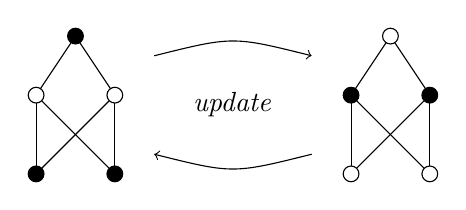
\begin{tikzpicture}
    % Leftmost graph:
    \draw (0,1) -- (0,0);
    \draw (1,1) -- (1,0);
    \draw (0,1) -- (1,0);
    \draw (1,1) -- (0,0);
    \draw (0.5,1.75) -- (0,1);
    \draw (0.5,1.75) -- (1,1);
    \filldraw[fill=black] (0.5,1.75) circle (0.1);
    \filldraw[fill=black] (0,0) circle (0.1);
    \filldraw[fill=white] (0,1) circle (0.1);
    \filldraw[fill=black] (1,0) circle (0.1);
    \filldraw[fill=white] (1,1) circle (0.1);

    % Rightmost graph:
    \draw (4,1) -- (4,0);
    \draw (5,1) -- (5,0);
    \draw (4,1) -- (5,0);
    \draw (5,1) -- (4,0);
    \draw (4.5,1.75) -- (4,1);
    \draw (4.5,1.75) -- (5,1);
    \filldraw[fill=white] (4.5,1.75) circle (0.1);
    \filldraw[fill=white] (4,0) circle (0.1);
    \filldraw[fill=black] (4,1) circle (0.1);
    \filldraw[fill=white] (5,0) circle (0.1);
    \filldraw[fill=black] (5,1) circle (0.1);

    % Update function arrows:
    \draw[->] (1.5,1.5) .. controls (2.5,1.75) .. (3.5,1.5);
    \draw[<-] (1.5,0.25) .. controls (2.5,0) .. (3.5,0.25);
    \draw (2.5,0.875) node {\emph{update}};
  \end{tikzpicture}
\end{center}

For simplicity, we will focus on the version of the model with two players, represented by the colours black and white. Nevertheless, the model hides a surprising amount of complexity. For instance, if one takes any finite black/white labelled graph and repeatedly applies the update function to it, one of three things eventually happens:

\begin{enumerate}
  \item The graph becomes monochromatic, i.e. one of the players wins.
  \item The graph is locked in a single state with both black and white vertices, i.e., there is a `static' stalemate.
  \item The graph settles into a periodic cycle, i.e. the same states keep occurring.
\end{enumerate}

The example we drew above is a periodic cycle of length $2$, since applying the update function repeatedly just alternates between the two graphs. In fact, \emph{every} case of a periodic cycle we've managed to come up with has length $2$! This leads us to conjecture that $2$ is the only possible length for a periodic cycle on a finite graph, but to date we have been unable to prove this.

%%%%%%%%%%%%%%%%%%%%%%%%%%%%%%%%%%%%%%%%%%%%%%%%%%%%%%%%%%%%%%%%%%%%%%%%%%%
\section{Choosing the Rules}
%%%%%%%%%%%%%%%%%%%%%%%%%%%%%%%%%%%%%%%%%%%%%%%%%%%%%%%%%%%%%%%%%%%%%%%%%%%

\newcommand{\selfDef}{\textsc{Sd}}
\newcommand{\nselfDef}{\neg \textsc{Sd}}
\newcommand{\tieNeu}{\textsc{Neu}}
\newcommand{\ntieNeu}{\neg \textsc{Neu}}

The main intuition we want to capture is that a vertex changes colour whenever its neighbourhood contains more \emph{enemies} than \emph{allies}. This raises (at least) two questions about the specifics of the update function:

\begin{enumerate}
  \item Does the vertex itself count as an allie? (``\emph{self-defence}'')
  \item What happens in the event of a tie? (``\emph{tie-breaking}'')
\end{enumerate}

Each of these questions leads to two obvious choices, for a total of four possible update functions. In the case of self-defence, we can either decide that a vertex \emph{does} count as its own allie (denoted $\selfDef$), or that it \emph{doesn't} count as its own allie (denoted $\nselfDef$). In the case of tie-breaking, we can either decide that a tied vertex becomes \emph{neutral} (i.e. owned by nobody, denoted $\tieNeu$), or that it simply stays the \emph{same} colour (denoted $\ntieNeu$).

The four combinations are then $\selfDef \wedge \tieNeu$, $\selfDef \wedge \ntieNeu$, $\nselfDef \wedge \tieNeu$ and $\nselfDef \wedge \ntieNeu$. To decide which of these combinations is the most natural, we look at what happens when we update the simplest possible black/white coloured graph according to these rules:

\begin{center}
  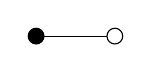
\begin{tikzpicture}
    \draw (0,0) -- (1,0);
    \filldraw[fill=black] (0,0) circle (0.1);
    \filldraw[fill=white] (1,0) circle (0.1);
  \end{tikzpicture}
\end{center}

\begin{center}
  \begin{tabular}{c|c|c|}
    \multicolumn{1}{c}{} &
    \multicolumn{1}{c}{$\selfDef$} &
    \multicolumn{1}{c}{$\nselfDef$} \\ 
    \cline{2-3}
    $\tieNeu$ &
    
    \begin{tikzpicture}
      \draw[fill=white,white] (-1, -1) rectangle (2, 1);
      \draw (0,0) -- (1,0);
      \filldraw[fill=gray] (0,0) circle (0.1);
      \filldraw[fill=gray] (1,0) circle (0.1);
    \end{tikzpicture} &

    \begin{tikzpicture}
      \draw[fill=white,white] (-1, -1) rectangle (2, 1);
      \draw (0,0) -- (1,0);
      \filldraw[fill=white] (0,0) circle (0.1);
      \filldraw[fill=black] (1,0) circle (0.1);
    \end{tikzpicture} \\

    \cline{2-3}
    $\ntieNeu$ &

    \begin{tikzpicture}
      \draw[fill=white,white] (-1, -1) rectangle (2, 1);
      \draw (0,0) -- (1,0);
      \filldraw[fill=black] (0,0) circle (0.1);
      \filldraw[fill=white] (1,0) circle (0.1);
    \end{tikzpicture} &

    \begin{tikzpicture}
      \draw[fill=white,white] (-1, -1) rectangle (2, 1);
      \draw (0,0) -- (1,0);
      \filldraw[fill=white] (0,0) circle (0.1);
      \filldraw[fill=black] (1,0) circle (0.1);
    \end{tikzpicture} \\

    \cline{2-3}
  \end{tabular}
\end{center}

%%%%%%%%%%%%%%%%%%%%%%%%%%%%%%%%%%%%%%%%%%%%%%%%%%%%%%%%%%%%%%%%%%%%%%%%%%%
\section{Notation}
%%%%%%%%%%%%%%%%%%%%%%%%%%%%%%%%%%%%%%%%%%%%%%%%%%%%%%%%%%%%%%%%%%%%%%%%%%%

%%%%%%%%%%%%%%%%%%%%%%%%%%%%%%%%%%%%%%%%%%%%%%%%%%%%%%%%%%%%%%%%%%%%%%%%%%%
\section{Basic definitions}
%%%%%%%%%%%%%%%%%%%%%%%%%%%%%%%%%%%%%%%%%%%%%%%%%%%%%%%%%%%%%%%%%%%%%%%%%%%
%This probably overlaps monstrously with the planned notation section, and what it has in brevity of definitions it somewhat lacks in clarity and quality XD

Let $G = (V,E)$ be a graph of order $n$. If $S$ be a subset of $V$, then $\ol{S} = V-S$ denotes the \textbf{complement} of $S$. Define the number $\epsilon_G$ (or just $\epsilon$ if the graph is clear from context) as $\epsilon_G = \frac{n}{n+1}$.

Let $G=(V,E)$ be a graph, and $f: \N \rightarrow \PS(V)$ a function. For a vertex $u$ and a natural number (henceforth called a \textbf{time}) $t$, \textbf{Bob's control of} \bm{$u$} \textbf{at time} \bm{$t$}, denoted \bm{$b_f(u, t)$}, is defined as
\[
b_f(u,t) = 
\begin{cases}
	|N[u] \cap f(t)| &\text{ if } u\notin f(t)\\
	|N[u] \cap f(t)| + \epsilon &\text{ if } u\in f(t)\\
\end{cases}
\]

Analogously, we define \textbf{Willow's control of} \bm{$u$} \textbf{at time} \bm{$t$}, denoted \bm{$w_f(u, t)$} as
\[
w_f(u,t) = 
\begin{cases}
|N[u] \cap \ol{f(t)}| &\text{ if } u\notin \ol{f(t)}\\
|N[u] \cap \ol{f(t)}| + \epsilon &\text{ if } u\in \ol{f(t)}\\
\end{cases}
\]

We will omit the subscript $f$ if the function is clear from context.
Since the vertex $u$ lies in either $f(t)$ or $\ol{f(t)}$, we have $b(u,t) + w(u,t) = |V| + \epsilon$.

A \textbf{dynamics} $f$ on $G$ is a function $f: \N \rightarrow \PS(V)$ such that for all $t \in \N$, and all $u\in V$, we have $u\in f(t+1)$ if and only if $b_f(u,t) > w_f(u,t)$. Dynamics are deterministic, in the sense that a dynamics $f$ is entirely determined by its \textbf{initial condition}, which is the set $f(0)$. Dynamics are \textbf{time-invariant}. If $f$ and $g$ are two dynamics on the same graph, and there exist times $s$ and $t$ such that $f(s) = g(t)$, then $f(s + k) = g(t + k)$ for all $k\in \N$. Finally, dynamics are symmetric in the role that Bob and Willow's vertices play. Instead of using the dynamics $f$ that provides the set of vertices under Bob's control, we could use the function $\overline{f}$, defined by $\overline{f}(t) = \overline{f(t)}$ for all $t\in \N$, which provides the set of vertices under Willow's control. Importantly, this new function $\ol{f}$ is itself a dynamics.

%%%%%%%%%%%%%%%%%%%%%%%%%%%%%%%%%%%%%%%%%%%%%%%%%%%%%%%%%%%%%%%%%%%%%%%%%%%
\section{Basic Results}
%%%%%%%%%%%%%%%%%%%%%%%%%%%%%%%%%%%%%%%%%%%%%%%%%%%%%%%%%%%%%%%%%%%%%%%%%%%

\begin{lem}[The Monotonicity Lemma]
	Let $G$ be a graph, and let $f$ and $g$ be two dynamics on $G$. 
	If there is some time $s$ such that $f(s) \subseteq g(s)$, then for all $s \leq t$, $f(t) \subseteq g(t)$.
	\label{lem_monotonicity_lem}
\end{lem}

\begin{proof}
	It suffices to prove that if $f(t) \subseteq g(t)$ for any time $t$, then $f(t+1) \subseteq g(t+1)$.
	
	Let $u$ be any vertex of $f(t+1)$. 
	Then $b_f(u,t) > w_f(u,t)$.
	Since $f(t) \subseteq g(t)$, we get the following chain of inequalities
	\[
		b_g(u,t) \geq b_f(u,t) > w_f(u,t) \geq w_g(u,t).
	\] 
	Therefore $u\in g(t+1)$.
\end{proof}

%%%%%%%%%%%%%%%%%%%%%%%%%%%%%%%%%%%%%%%%%%%%%%%%%%%%%%%%%%%%%%%%%%%%%%%%%%%
\section{Strongholds, victory and resistance}
%%%%%%%%%%%%%%%%%%%%%%%%%%%%%%%%%%%%%%%%%%%%%%%%%%%%%%%%%%%%%%%%%%%%%%%%%%%

Let $G = (V,E)$ be a graph, $S$ a subset of $V$, and $f$ a dynamics on $G$. The set $S$ is:
\begin{itemize}
	\item a \textbf{stronghold} if $f(0) = S$ implies that, for all $t\in \N$, $S \subseteq f(t)$.
	\item a \textbf{resistance set} if $f(0) = S$ implies that, for all $t\in \N$, $f(t) \neq \emptyset$.
	\item a \textbf{victory set} if $f(0) = S$ implies that there exists $t\in \N$ such that $f(t) = V$.
\end{itemize}

The \textbf{stronghold number} of $G$, denoted $\sigma_s(G)$, is the minimum number of vertices in a persistent set. The \textbf{resistance number} $\sigma_r(G)$ and \textbf{victory number} $\sigma_v(G)$ are defined analogously. There are some easily established relationships between these parameters.

\begin{prop}
	Let $G$ be a graph of order $n$ with stronghold, resistance and victory numbers $\sigma_s, \sigma_r$ and $\sigma_v$ respectively. Then:
	\begin{itemize}
		\item[(1)] $\sigma_r \leq \sigma_s$,
		\item[(2)] $\sigma_r \leq \sigma_v \leq n+1 - \sigma_r$,
		\item[(3)] $\sigma_r \leq \frac{n+1}{2}$
	\end{itemize}
	For arbitrary graphs, these bounds are all sharp.
	\label{prop_sigma_bounds}
\end{prop}

\begin{proof}
	Inequality (1) follows from the fact that every stronghold is a resistance set.
	
	To obtain the left hand side of (2), observe that every victory set is a resistance set. 
	If $S$ is not a resistance set, then its complement $\ol{S}$ is a victory set. Therefore every set containing at least $n-\sigma_r + 1$ vertices is a victory set --- yielding the right hand side of (2).
	
	To obtain inequality (3), add $\sigma_r$ to every term of (2), then divide by 2.
	
	Let $m$ be an odd natural number. Then $\sigma_s(K_m) = \sigma_r(K_m) = \sigma_v(K_m) = \frac{m+1}{2}$, demonstrating that all of the bounds are sharp for infinitely many graphs.
\end{proof}

If $u$ is a vertex of degree 1, then $\{u\}$ is a stronghold. Thus, if $G$ is a graph with $\delta(G) = 1$ (such as tree), then $\sigma_s(G) = \sigma_r(G) = 1$. However, it's possible for Bob to (eventually) control an entire tree by picking an initial condition $f(0)$ with far fewer than $n$ vertices.

%%%%%%%%%%%%%%%%%%%%%%%%%%%%%%%%%%%%%%%%%%%%%%%%%%%%%%%%%%%%%%%%%%%%%%%%%%%
\bibliographystyle{unsrt}
\bibliography{bibliography}
%%%%%%%%%%%%%%%%%%%%%%%%%%%%%%%%%%%%%%%%%%%%%%%%%%%%%%%%%%%%%%%%%%%%%%%%%%%

%%%%%%%%%%%%%%%%%%%%%%%%%%%%%%%%%%%%%%%%%%%%%%%%%%%%%%%%%%%%%%%%%%%%%%%%%%%
\end{document}
%%%%%%%%%%%%%%%%%%%%%%%%%%%%%%%%%%%%%%%%%%%%%%%%%%%%%%%%%%%%%%%%%%%%%%%%%%%
